\documentclass{article}

\usepackage{ctex}
\usepackage[top=0.7in,bottom=0.7in,left=0.5in,right=0.5in]{geometry}
\usepackage{array}
\usepackage{multirow}
\usepackage{graphicx}
\usepackage{subfigure}
\usepackage{fancyhdr}
\usepackage{lastpage}
\usepackage{extramarks}
\usepackage{amsmath}
\usepackage{listings}
\usepackage{fontspec}
\newfontfamily\consolas{Consolas}
\usepackage{xcolor} % 定制颜色
\definecolor{mygreen}{rgb}{0,0.6,0}
\definecolor{mygray}{rgb}{0.5,0.5,0.5}
\definecolor{mymauve}{rgb}{0.58,0,0.82}
\lstset{ %
backgroundcolor=\color{white},      % choose the background color
basicstyle=\footnotesize\ttfamily,  % size of fonts used for the code
columns=fullflexible,
tabsize=4,
breaklines=true,               % automatic line breaking only at whitespace
captionpos=b,                  % sets the caption-position to bottom
commentstyle=\color{mygreen},  % comment style
escapeinside={\%*}{*)},        % if you want to add LaTeX within your code
keywordstyle=\color{blue},     % keyword style
stringstyle=\color{mymauve}\ttfamily,  % string literal style
frame=single,
rulesepcolor=\color{red!20!green!20!blue!20},
% identifierstyle=\color{red},
language=c++,
}

\newcommand{\hmwkTitle}{哈夫曼编码压缩、解压文件\ 实验报告}
\newcommand{\hmwkClass}{数据结构}
\newcommand{\hmwkClassInstructor}{}
\newcommand{\hmwkAuthorName}{毛子恒\ 李臻\ 张梓靖}

\pagestyle{fancy}
\lhead{\hmwkAuthorName}
\chead{\hmwkClass\ : \hmwkTitle}
\rhead{\firstxmark}
\lfoot{\lastxmark}
\cfoot{\thepage}
\renewcommand\headrulewidth{0.4pt}
\renewcommand\footrulewidth{0.4pt}

\title{\hmwkClass\ :\hmwkTitle}
\author{\hmwkAuthorName}

\setcounter{tocdepth}{1}

\begin{document}

\maketitle

\section*{小组成员}

\setlength{\tabcolsep}{9mm}
{
    \begin{table}[htbp]
        \centering
        \begin{tabular}{llll}
            班级:2019211309 & 姓名:毛子恒 & 学号:2019211397 & 分工:代码\ 文档   \\

            班级:2019211310 & 姓名:李臻   & 学号:2019211458 & 分工:测试\ 文档   \\

            班级:2019211308 & 姓名:张梓靖 & 学号:2019211379 & 分工:可视化\ 文档 \\
        \end{tabular}
    \end{table}
}

\tableofcontents
\newpage

\section{需求分析}

\subsection{题目描述}

对于一个指定的文件,应用哈夫曼编码压缩文件,或者对本程序生成的压缩文件进行解压。

\subsection{输入描述}

程序从标准输入中读入数据。

输入一行两个整数$n,m$($n>0,m>0$),用空格分隔,分别表示A矩阵的行数和列数。

之后的$n$行,每行$m$个整数,用空格分隔,表示A矩阵。

之后的若干行为B矩阵的信息,格式相同。

\subsection{输出描述}

程序向标准输出中输出结果。

输出分为五种情况:

\begin{enumerate}
    \item 输入合法,两个矩阵可以相加、相乘,程序正常运行结束。此时输出矩阵运算的结果。
    \item 矩阵不能相加,此时没有相加的结果,输出一行一个字符串"Cannot add matrix A and B, An != Bn."或"Cannot add matrix A and B, Am != Bm."或"Cannot add matrix A and B, An != Bn, Am != Bm."(不含引号)
    \item 矩阵不能相乘,此时没有相乘的结果,输出一行一个字符串"Cannot multiply matrix A and B, Am != Bn."(不含引号)
    \item $n$或$m$的范围不合法,此时输出一行一个字符串"Please check your input."(不含引号)
    \item 程序发生运行时错误,比如内存分配失败。此时程序没有输出。
\end{enumerate}

\subsection{样例输入输出}

\subsubsection{样例输入输出1}

【输入】

\begin{lstlisting}[
    basicstyle=\small\consolas]
2 2
3 0
0 7
2 2
4 6
0 8
\end{lstlisting}

【输出】

\begin{lstlisting}[
    basicstyle=\small\consolas]
7 6 
0 15 
12 18 
0 56 
\end{lstlisting}

\subsubsection{样例输入输出2}

【输入】

\begin{lstlisting}[
    basicstyle=\small\consolas]
8 8
282 0 708 0 449 0 0 39
685 79 0 0 385 0 638 0
745 0 244 0 658 795 0 0
923 985 0 0 0 0 152 0
602 167 0 0 0 143 0 0
568 233 35 0 0 0 0 0
0 0 284 0 310 23 0 625
542 0 303 293 286 0 387 510
8 8
578 781 779 0 0 0 0 0
0 531 0 940 106 464 0 735
346 141 287 273 0 746 804 665
917 0 0 0 0 0 409 788
0 0 176 784 0 383 13 879
927 881 899 146 118 0 0 709
42 84 0 254 0 0 90 0
552 0 0 955 0 0 0 0
\end{lstlisting}

【输出】

\begin{lstlisting}[
    basicstyle=\small\consolas]
860 781 1487 0 449 0 0 39 
685 610 0 940 491 464 638 735 
1091 141 531 273 658 1541 804 665 
1840 985 0 0 0 0 561 788 
602 167 176 784 0 526 13 879 
1495 1114 934 146 118 0 0 709 
42 84 284 254 310 23 90 625 
1094 0 303 1248 286 0 387 510 
429492 320070 501898 582545 0 700135 575069 865491 
422726 630526 601375 538152 8374 184111 62425 396480 
1251999 1316644 1480896 698554 93810 434038 204730 1304297 
539878 1256666 719017 964508 104410 457040 13680 723975 
480517 684822 597515 177858 34576 77488 0 224132 
340414 572266 452517 228575 24698 134222 28140 194530 
464585 60307 156745 920805 2714 330594 232366 477657 
984569 498533 559515 892291 0 335576 401997 683773
\end{lstlisting}

\subsubsection{样例输入输出3}

【输入】

\begin{lstlisting}[
    basicstyle=\small\consolas]
2 3
1 6 0
3 0 7
3 1
5
0
8
\end{lstlisting}

【输出】

\begin{lstlisting}[
    basicstyle=\small\consolas]
Cannot add matrix A and B, An != Bn, Am != Bm.
5 
71 
\end{lstlisting}

\subsubsection{样例输入输出4}

【输入】

\begin{lstlisting}[
    basicstyle=\small\consolas]
4 2
2 5
0 3
2 0
7 0
1 3
1 0 6
\end{lstlisting}

【输出】

\begin{lstlisting}[
    basicstyle=\small\consolas]
Cannot add matrix A and B, An != Bn, Am != Bm.
Cannot multiply matrix A and B, Am != Bn.
\end{lstlisting}

\subsection{程序功能}

程序判别两个矩阵能否相加/相乘,并完成计算。

\section{概要设计}

\subsection{问题解决的思路}

使用三元组表存储稀疏矩阵,并且设计三元组表形式的矩阵加法和乘法算法、一维数组存储的矩阵和三元组表存储的矩阵之间的转化算法。

\subsection{矩阵的定义}

\begin{lstlisting}[language={C},
    numbers=left,
    numberstyle=\tiny\consolas,
    basicstyle=\small\consolas]
//数据对象
typedef struct
{
    int i, j;
    long long val;
} Tuple;

typedef struct
{
    Tuple * data;
    int * pos; // 每一行中首个非零元素的位置
    int n, m, tot; // tot为非空元素总数
    int sizeOfMatrix; // 三元组存储单位的个数
} Matrix;

/*
 * 操作:初始化矩阵
 * 前件:a指向一个空矩阵,n>0,m>0
 * 后件:a指向一个n*m的零矩阵
 */
void initMatrix(Matrix * a, int n, int m);

/*
 * 操作:扩展矩阵的存储空间
 * 前件:c指向一个矩阵
 * 后件:该矩阵扩展MATRIXINCREASESIZE个三元组存储单位
 */
void expandMatrix(Matrix * c);

/*
 * 操作:把由一维数组存储的矩阵转化为由三元组表存储的矩阵
 * 前件:n>0,m>0,val中存储一个矩阵,矩阵元素a[i][j]存储在val[(i-1)*m+j]中
 * 后件:函数返回由三元组表作为存储形式的矩阵
 */
Matrix array2Matrix(int n, int m, long long val[]);

/*
 * 操作:把两个矩阵相加
 * 前件:a,b为两个矩阵,并且行数和列数都相等
 * 后件:函数返回两个矩阵相加的结果
 */
Matrix addMatrix(Matrix a, Matrix b);

/*
 * 操作:把两个矩阵相乘
 * 前件:a,b为两个矩阵,并且a的列数和b的行数相等
 * 后件:函数返回两个矩阵相乘的结果
 */
Matrix mulMatrix(Matrix a, Matrix b);

/*
 * 操作:把由三元组表存储的矩阵转化为由一维数组存储的矩阵
 * 前件:a为一个矩阵,val指向一个至少有n*m+1个存储单位的long long类型的数组
 * 后件:val指向由一维数组存储的矩阵,矩阵元素a[i][j]存储在val[(i-1)*m+j]中
 */
void matrix2Array(Matrix a, long long val[]);

/*
 * 操作:释放矩阵空间
 * 前件:a指向一个矩阵
 * 后件:a指向一个空矩阵
 */
void destroyMatrix(Matrix * a);
\end{lstlisting}

\subsection{主程序的流程}

\begin{enumerate}
    \item 输入,矩阵存入一维数组
    \item 一维数组存储的矩阵转化为由三元组表存储的矩阵
    \item 判断矩阵能否相加
    \item 如果能,则相加,输出
    \item 判断矩阵能否相乘
    \item 如果能,则相乘,输出
    \item 释放空间
\end{enumerate}

\subsection{各程序模块之间的层次关系}

程序模块层次关系图如图1。

\begin{figure}[htbp]

    % \centering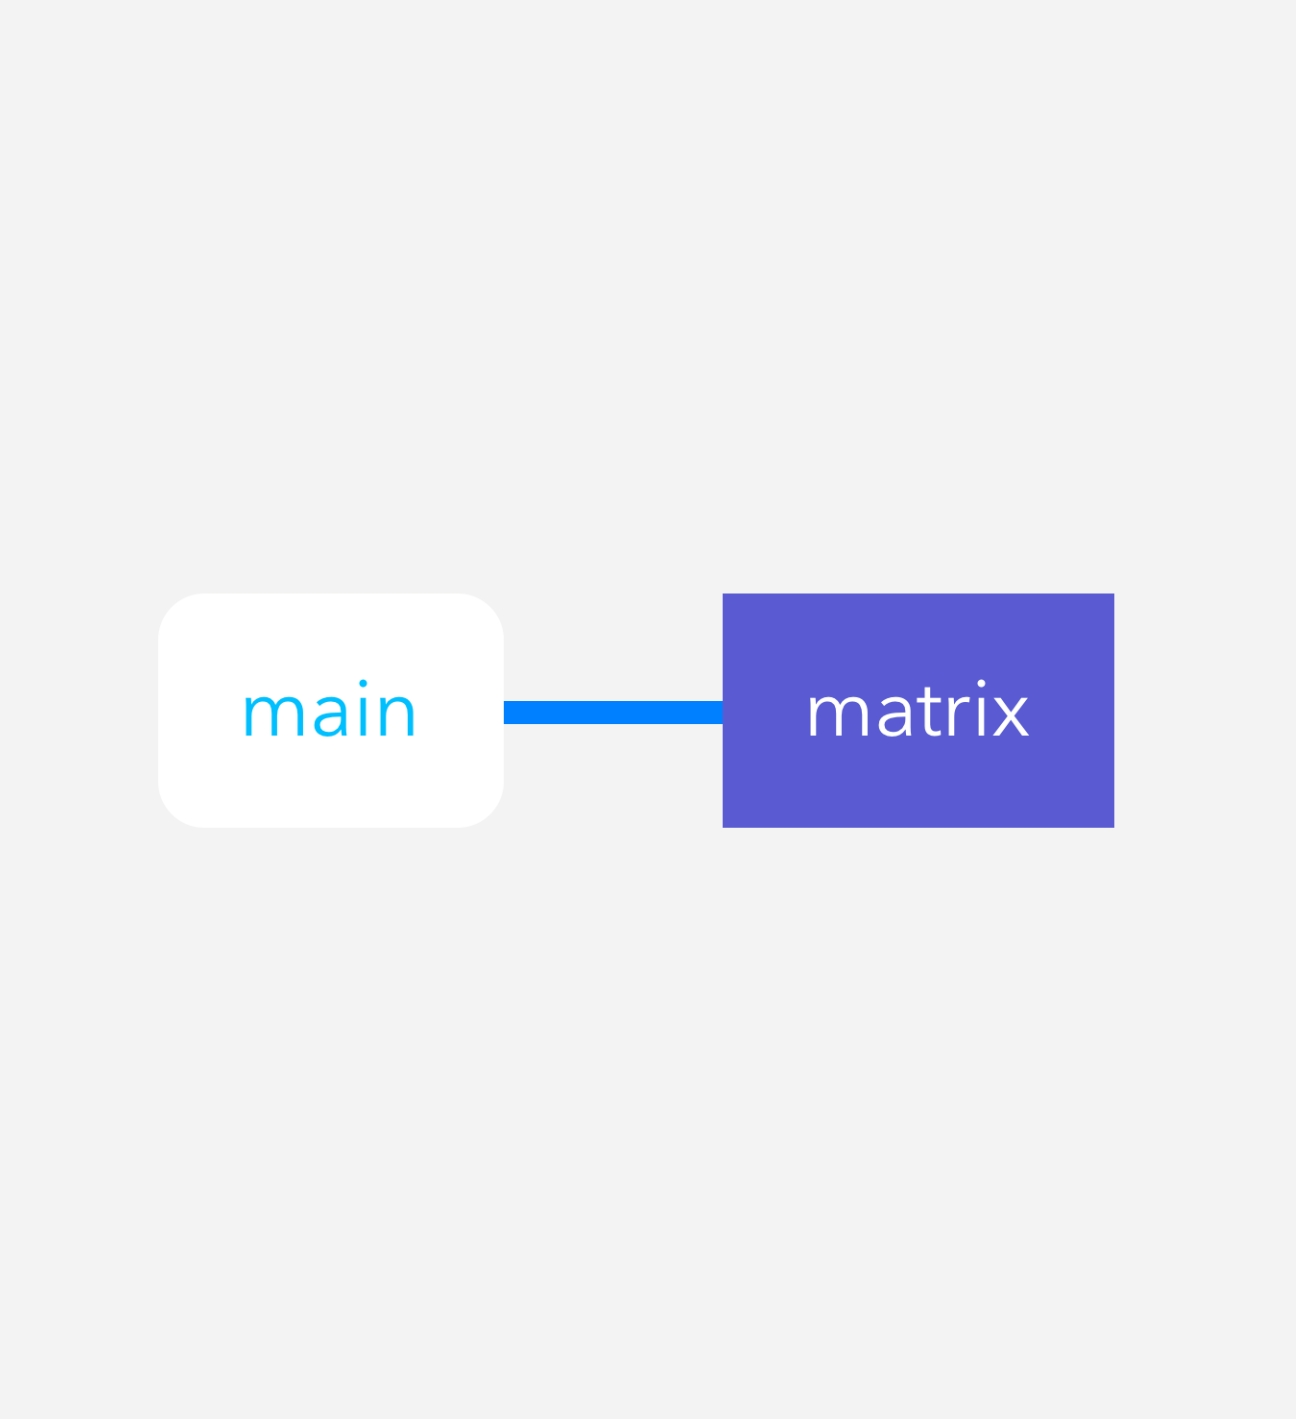
\includegraphics[width=0.4\textwidth]{./Images/pic3_1.png}

    \caption{程序模块层次关系}

\end{figure}

\section{详细设计}

\subsection{矩阵的实现}

矩阵的设计中基本操作的伪代码算法如下:

\begin{lstlisting}[language={C},
    numbers=left,
    numberstyle=\tiny\consolas,
    basicstyle=\small\consolas]
// 初始化矩阵
void initMatrix(Matrix * a, int n, int m)
{
    a->n <- n
    a->m <- m
    a->tot <- 0
    if (给a->pos分配内存失败)
        异常退出
    a->sizeOfMatrix <- MATRIXINCREASESIZE
    if (给a->data分配内存失败)
        异常退出
}
    
// 扩展矩阵的存储空间
void expandMatrix(Matrix * c)
{
    if (给c->data分配内存失败)
        异常退出
    c->sizeOfMatrix <- c->sizeOfMatrix + MATRIXINCREASESIZE
}

// 把由一维数组存储的矩阵转化为由三元组表存储的矩阵
Matrix array2Matrix(int n, int m, long long val[])
{
    定义矩阵a并初始化
    for (i = 1 to n)
    {
        a.pos[i] <- a.tot + 1
        for (j = 1 to m)
        {
            if (val[(i - 1) * m + j]不为零)
            {
                if (矩阵a的存储空间不足)
                    扩展矩阵a的存储空间
                a.data[++a.tot] <- (Tuple) {i, j, val[(i - 1) * m + j]}
            }
        }
    }
    a.pos[n + 1] <- a.tot + 1
    返回a
}

// 两个矩阵相加
Matrix addMatrix(Matrix a, Matrix b)
{
    if (两个矩阵的行列大小不相等) 
        异常退出
    定义矩阵c并初始化
    if (有一个矩阵为空)
        返回空矩阵c
    for (i = 1 to a.n)
    {
        c.pos[i] <- c.tot + 1
        p1 <- a.pos[i] 
        p2 <- b.pos[i]
        while (p1 < a.pos[i + 1] 或 p2 < b.pos[i + 1]) // 枚举a矩阵和b矩阵第i行的非零元素
        {
            定义tempj,tempy // 用于记录c矩阵中每一个位置加法的结果
            if (b矩阵本行没有元素 或 a矩阵非零元素列数小于b矩阵非零元素的列数) 
            {
                tempj <- a.data[p1].j
                tempv <- a.data[p1].val
                ++p1
            }
            else if (a矩阵本行没有元素 或 b矩阵非零元素列数小于a矩阵非零元素的列数) 
            {
                tempj <- b.data[p2].j
                tempv <- b.data[p2].val
                ++p2
            }
            else 
            {
                tempj <- a.data[p1].j
                tempv <- a.data[p1].val + b.data[p2].val
                ++p1
                ++p2
            }
            if (c[i][j]不为0)
            {
                if (矩阵c存储空间不足)
                    扩展矩阵的存储空间
                c.data[++c.tot] <- (Tuple) {i, tempj, tempv}
            }
        }
    }
    c.pos[c.n + 1] <- c.tot + 1
    返回c
}

// 两个矩阵相乘
Matrix mulMatrix(Matrix a, Matrix b)
{
    if (第一个矩阵的列数不等于第二个矩阵的行数) // 两个矩阵不可相乘
        异常退出
    定义矩阵c并初始化
    if (有一个矩阵为空)
        返回空矩阵c
    定义临时数组temp并分配内存 // 临时数组,用于记录c矩阵中每一行的结果
    for (i = 1 to a.n)
    {
        temp数组清零
        c.pos[i] <- c.tot + 1
        for (p = a.pos[i] to a.pos[i + 1] - 1) // 枚举a矩阵第i行的非零元素
        {
            k <- a.data[p].j // a矩阵的该非零元素为a[i][k]
            for (q = b.pos[k] to b.pos[k + 1] - 1) // 枚举b矩阵第k行的非零元素
            {
                j <- b.data[q].j // b矩阵的该非零元素为b[k][j]
                temp[j] <- temp[j] + a.data[p].val * b.data[q].val
            }
        }
        for (j = 1 to b.m)
        {
            if (c[i][j]不等于0) 
            {
                if (矩阵c存储空间不足)
                    扩展矩阵的存储空间
                c.data[++c.tot] <- (Tuple) {i, tempj, tempv}
            }
        }
    }
    c.pos[c.n + 1] <- c.tot + 1
    释放temp
    返回c
}

// 把由三元组表存储的矩阵转化为由一维数组存储的矩阵
void matrix2Array(Matrix a, long long val[])
{
    val数组清零
    for (i = 1 to a.tot)
        val[(a.data[i].i - 1) * a.m + a.data[i].j] <- a.data[i].val; // a[i][j]存储在val[(i-1]*m+j]中
}

// 释放矩阵空间
void destroyMatrix(Matrix * a)
{
    释放a->pos
    释放a->data
    a->n <- 0
    a->m <- 0
    a->tot <- 0
    a->sizeOfMatrix <- 0
}
\end{lstlisting}

\subsection{函数的调用关系图}

函数调用关系图如图2。

\begin{figure}[htbp]

    % \centering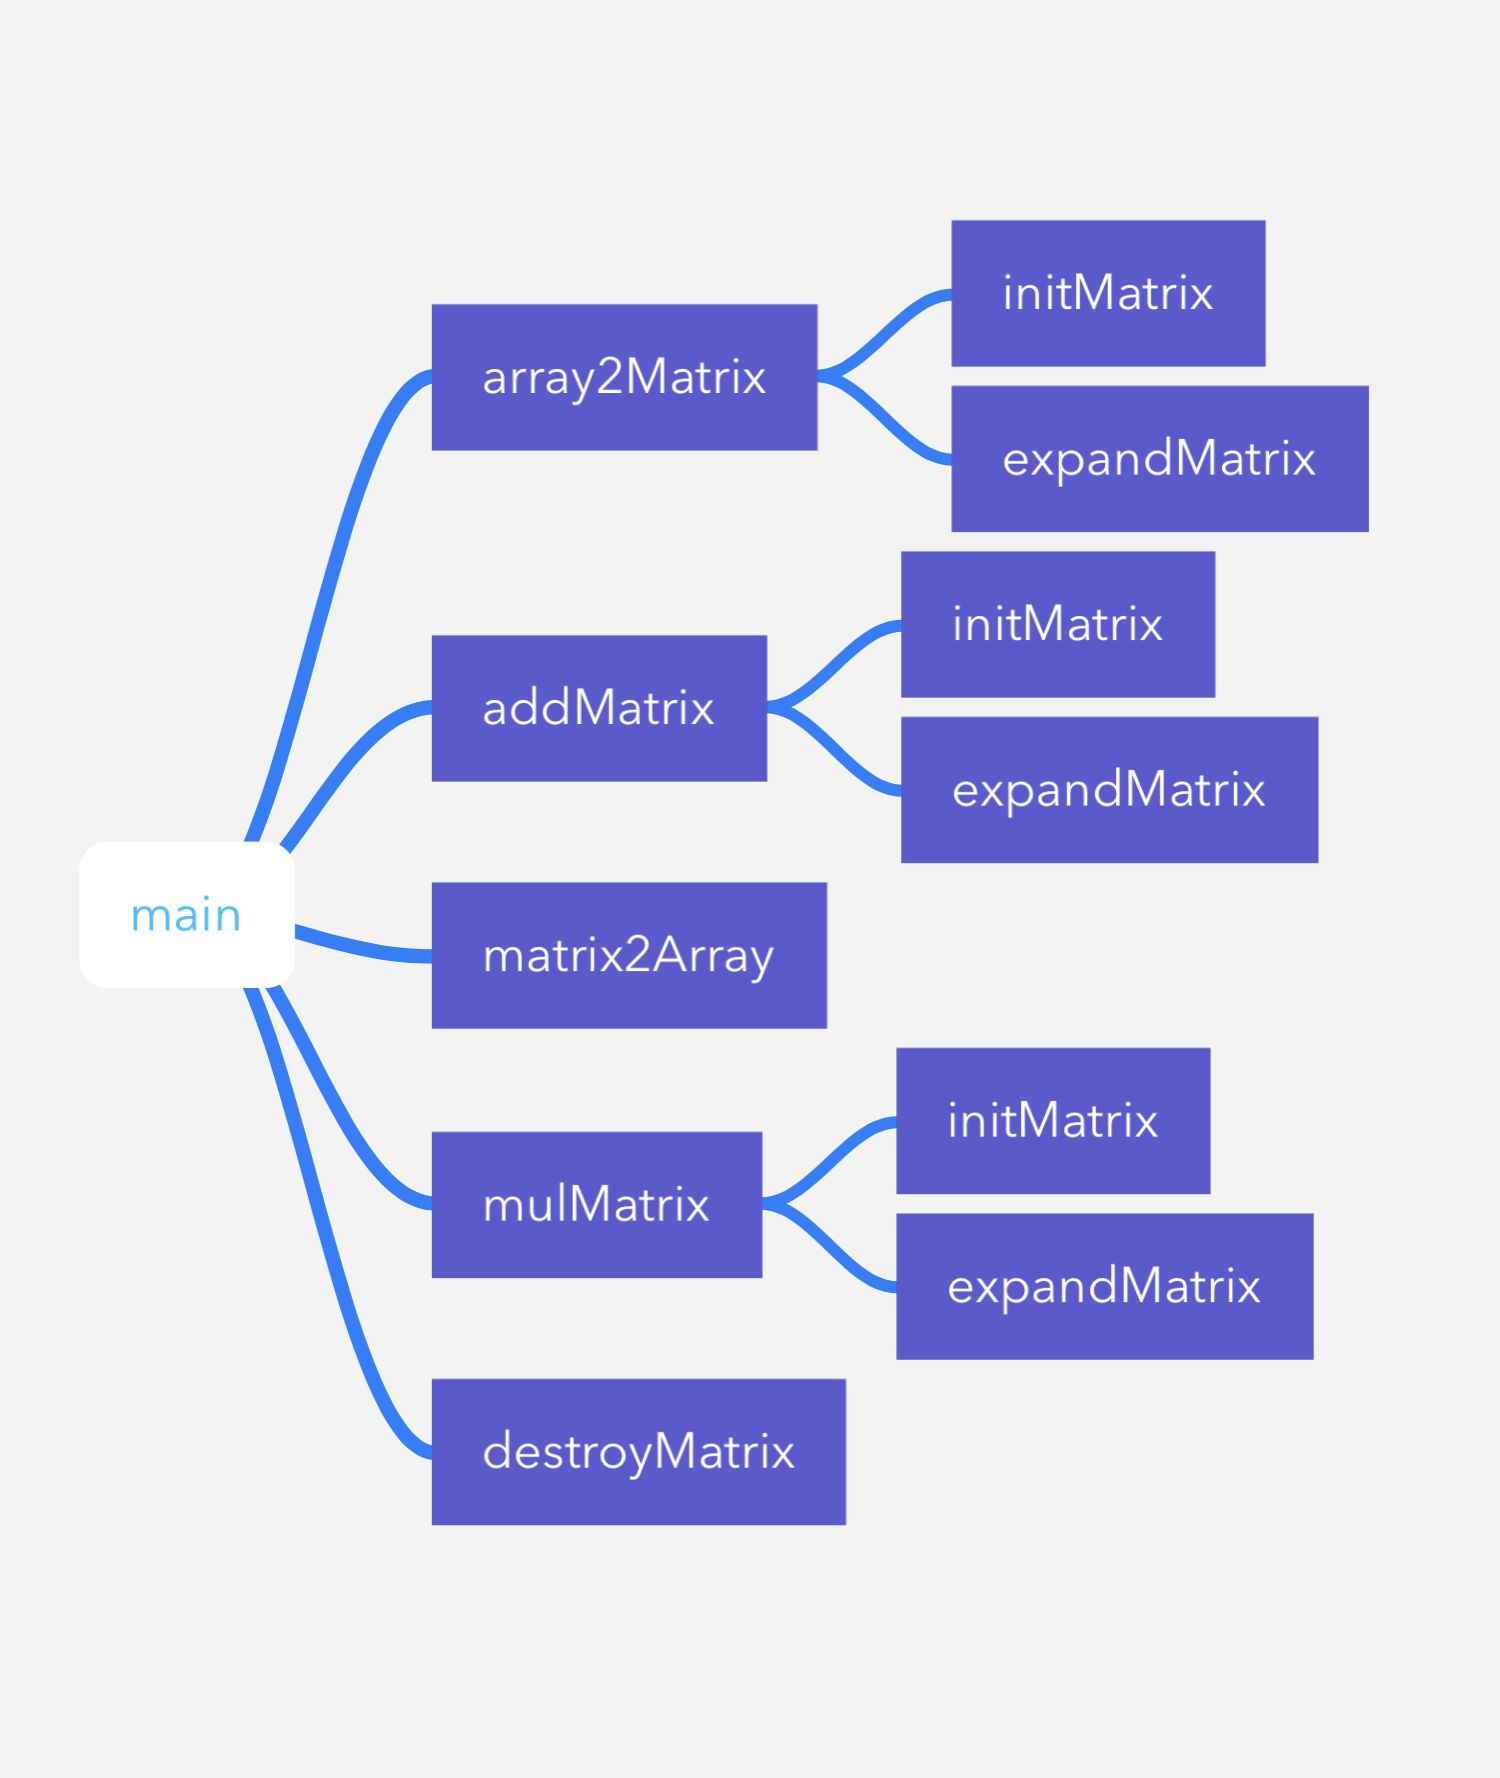
\includegraphics[width=0.4\textwidth]{./Images/pic3_2.png}

    \caption{函数调用关系图}

\end{figure}

\section{调试分析报告}

\subsection{调试过程中遇到的问题和思考}

程序在一些小细节中出现了问题,比如$val$数组需要多分配一个空间,矩阵相乘后$c$矩阵的列数等于$b$矩阵的列数。

初次实现矩阵相加算法时设计有误,使得两个矩阵的某个对应位置只要有一个为零,就会忽略这个位置,这个问题通过if判断修复。

在随机测试中发现数据规模较大时结果很容易超出int类型的范围,故矩阵元素采用long long类型。

\subsection{设计实现的回顾讨论}

由于二维数组的内存分配、函数传参较为复杂,所以输入、输出时使用一维数组存储的矩阵。

期望矩阵的规模不超过$10^3$,所以$MATRIXINCREASESIZE$常量的值设置为$10^5$。

\subsection{算法复杂度分析}

initMatrix, expandMatrix, destroyMatrix函数的复杂度为$O(1)$

array2Matrix, matrix2Array, addMatrix函数的复杂度为$O(n^2)$,mulMatrix函数的复杂度为$O(n^3)$,视矩阵的稀疏程度,算法的时间复杂度会有常数级别的优化。在本报告的最后部分有讨论。

主函数的时间复杂度为$O(n^2)$,整体时间复杂度为$O(n^3)$。

整体空间复杂度为$O(n^2)$。

\subsection{改进设想的经验和体会}

\subsubsection{改进1}

可以在输入/输出时简化数组存储的矩阵和三元组表存储的矩阵之间转化的过程,会有常数级别的优化。

\section{用户使用说明}

使用gcc编译生成可执行文件。

\begin{lstlisting}[language={bash},
    basicstyle=\small\consolas]
gcc -o main -std=c11 main.c matrix.c
\end{lstlisting}

执行可执行文件:

\begin{lstlisting}[language={bash},
    basicstyle=\small\consolas]
./main
\end{lstlisting}

在Windows cmd下:

\begin{lstlisting}[language={bash},
    basicstyle=\small\consolas]
main
\end{lstlisting}

之后通过标准输入输入数据,输入格式参考1.2节的输入描述,结果通过标准输出返回。如果输入合法并且程序正常运行结束,主函数返回值为0。

\section{测试结果}

测试环节分为三个步骤。

\subsection{测试第一部分}

对1.4节给出的样例进行测试。

\subsection{测试第二部分}

测试边界条件。

【输入】

\begin{lstlisting}[
    basicstyle=\small\consolas]
1 0
1 1
2
\end{lstlisting}

【输出】

\begin{lstlisting}[
    basicstyle=\small\consolas]
Please check your input.
\end{lstlisting}

【输入】

\begin{lstlisting}[
    basicstyle=\small\consolas]
4 3
7 0 6
0 0 5
1 0 0
0 0 2
3 3
5 7 0
0 3 0
1 3 5
\end{lstlisting}

【输出】

\begin{lstlisting}[
    basicstyle=\small\consolas]
Cannot add matrix A and B, An != Bn.
41 67 30 
5 15 25 
5 7 0 
2 6 10 
\end{lstlisting}

【输入】

\begin{lstlisting}[
    basicstyle=\small\consolas]
3 3
7 0 6
1 0 4
1 0 0
3 4
5 7 0 1
0 3 0 0
1 3 5 0
\end{lstlisting}

【输出】

\begin{lstlisting}[
    basicstyle=\small\consolas]
Cannot add matrix A and B, Am != Bm.
41 67 30 7 
9 19 20 1 
5 7 0 1 
\end{lstlisting}

【输入】

\begin{lstlisting}[
    basicstyle=\small\consolas]
3 4
7 0 6 4
1 0 4 0
1 0 0 6
3 4
5 7 0 1
0 3 0 0
1 3 5 0
\end{lstlisting}

【输出】

\begin{lstlisting}[
    basicstyle=\small\consolas]
12 7 6 5 
1 3 4 0 
2 3 5 6 
Cannot multiply matrix A and B, Am != Bn.
\end{lstlisting}

\subsection{测试第三部分}

将原解法与二维数组实现的矩阵加法和乘法(testing/test.c)比对。

测试在macOS\ Catalina\ 10.15.6下进行。

在$n<=10$,$n<=100$,$n<=1000$的范围下分别随机生成1000组测试数据,分别传入main和test,并且比对两程序的输出。

3000组数据中两程序的输出均相同。

数据生成程序(testing/data.cpp)如下:

\begin{lstlisting}[language={C++},
    numbers=left,
    numberstyle=\tiny\consolas,
    basicstyle=\small\consolas]
#include <bits/stdc++.h>
using namespace std;

const int SIZE = 1e3, PERCENT = 50;

int main()
{
    srand(time(0));
    int n = rand() % SIZE + 1;
    printf("%d %d\n", n, n);
    for (int i = 1; i <= n; ++i)
    {
        for (int j = 1; j <= n; ++j)
            printf("%d ", rand() % 100 > PERCENT ? 0 : rand() % 1000 + 1);
        puts("");
    }
    printf("%d %d\n", n, n);
    for (int i = 1; i <= n; ++i)
    {
        for (int j = 1; j <= n; ++j)
            printf("%d ", rand() % 100 > PERCENT ? 0 : rand() % 1000 + 1);
        puts("");
    }
    return 0;
}
\end{lstlisting}

比对脚本(testing/chk.sh)如下:

\begin{lstlisting}[language={bash},
    numbers=left,
    numberstyle=\tiny\consolas,
    basicstyle=\small\consolas]
for i in {1..1000}
do
    sleep 1
    ./data >in.in
    ./main <in.in >out.out
    ./test <in.in >out1.out
    if ! diff out.out out1.out
    then
        break
    fi
    echo "Correct"
done
\end{lstlisting}

\section{可视化}

随机生成若干组数据,由三元组表实现和二维数组实现分别计算,比对运行时间,并且使用JavaScript将结果可视化。

比对脚本(testing/timecount.py)如下:

\begin{lstlisting}[language={python},
    numbers=left,
    numberstyle=\tiny\consolas,
    basicstyle=\small\consolas]
import os
import json
import time
a = []
b = []
for i in range(100):
    os.system("./data >in.in")
    starttime = time.time()
    os.system("./main <in.in >out.out")
    endtime = time.time()
    a.append(endtime-starttime)
    starttime = time.time()
    os.system("./test <in.in >out1.out")
    endtime = time.time()
    b.append(endtime-starttime)
    print(i)

json_str = json.dumps([a, b])
with open("80%result.json", mode="w") as file:
    file.write(json_str)
\end{lstlisting}

数据规模如下:

$n=1000$,$20\%$的元素是0、$50\%$的元素是0、$80\%$的元素是0的数据各100组,共300组数据。

\subsubsection{实现细节}

利用已有的时间数据,使用Highcharts库绘制二维柱状图,比较两种算法的运行时间差距。

\subsubsection{用户使用说明}

使用现代浏览器打开Chart/index.html,即可看到柱状图,将鼠标指针放到某个柱上可以看到对应的值。

\subsubsection{示例}

见图3。

\begin{figure}[htbp]
    
    % \centering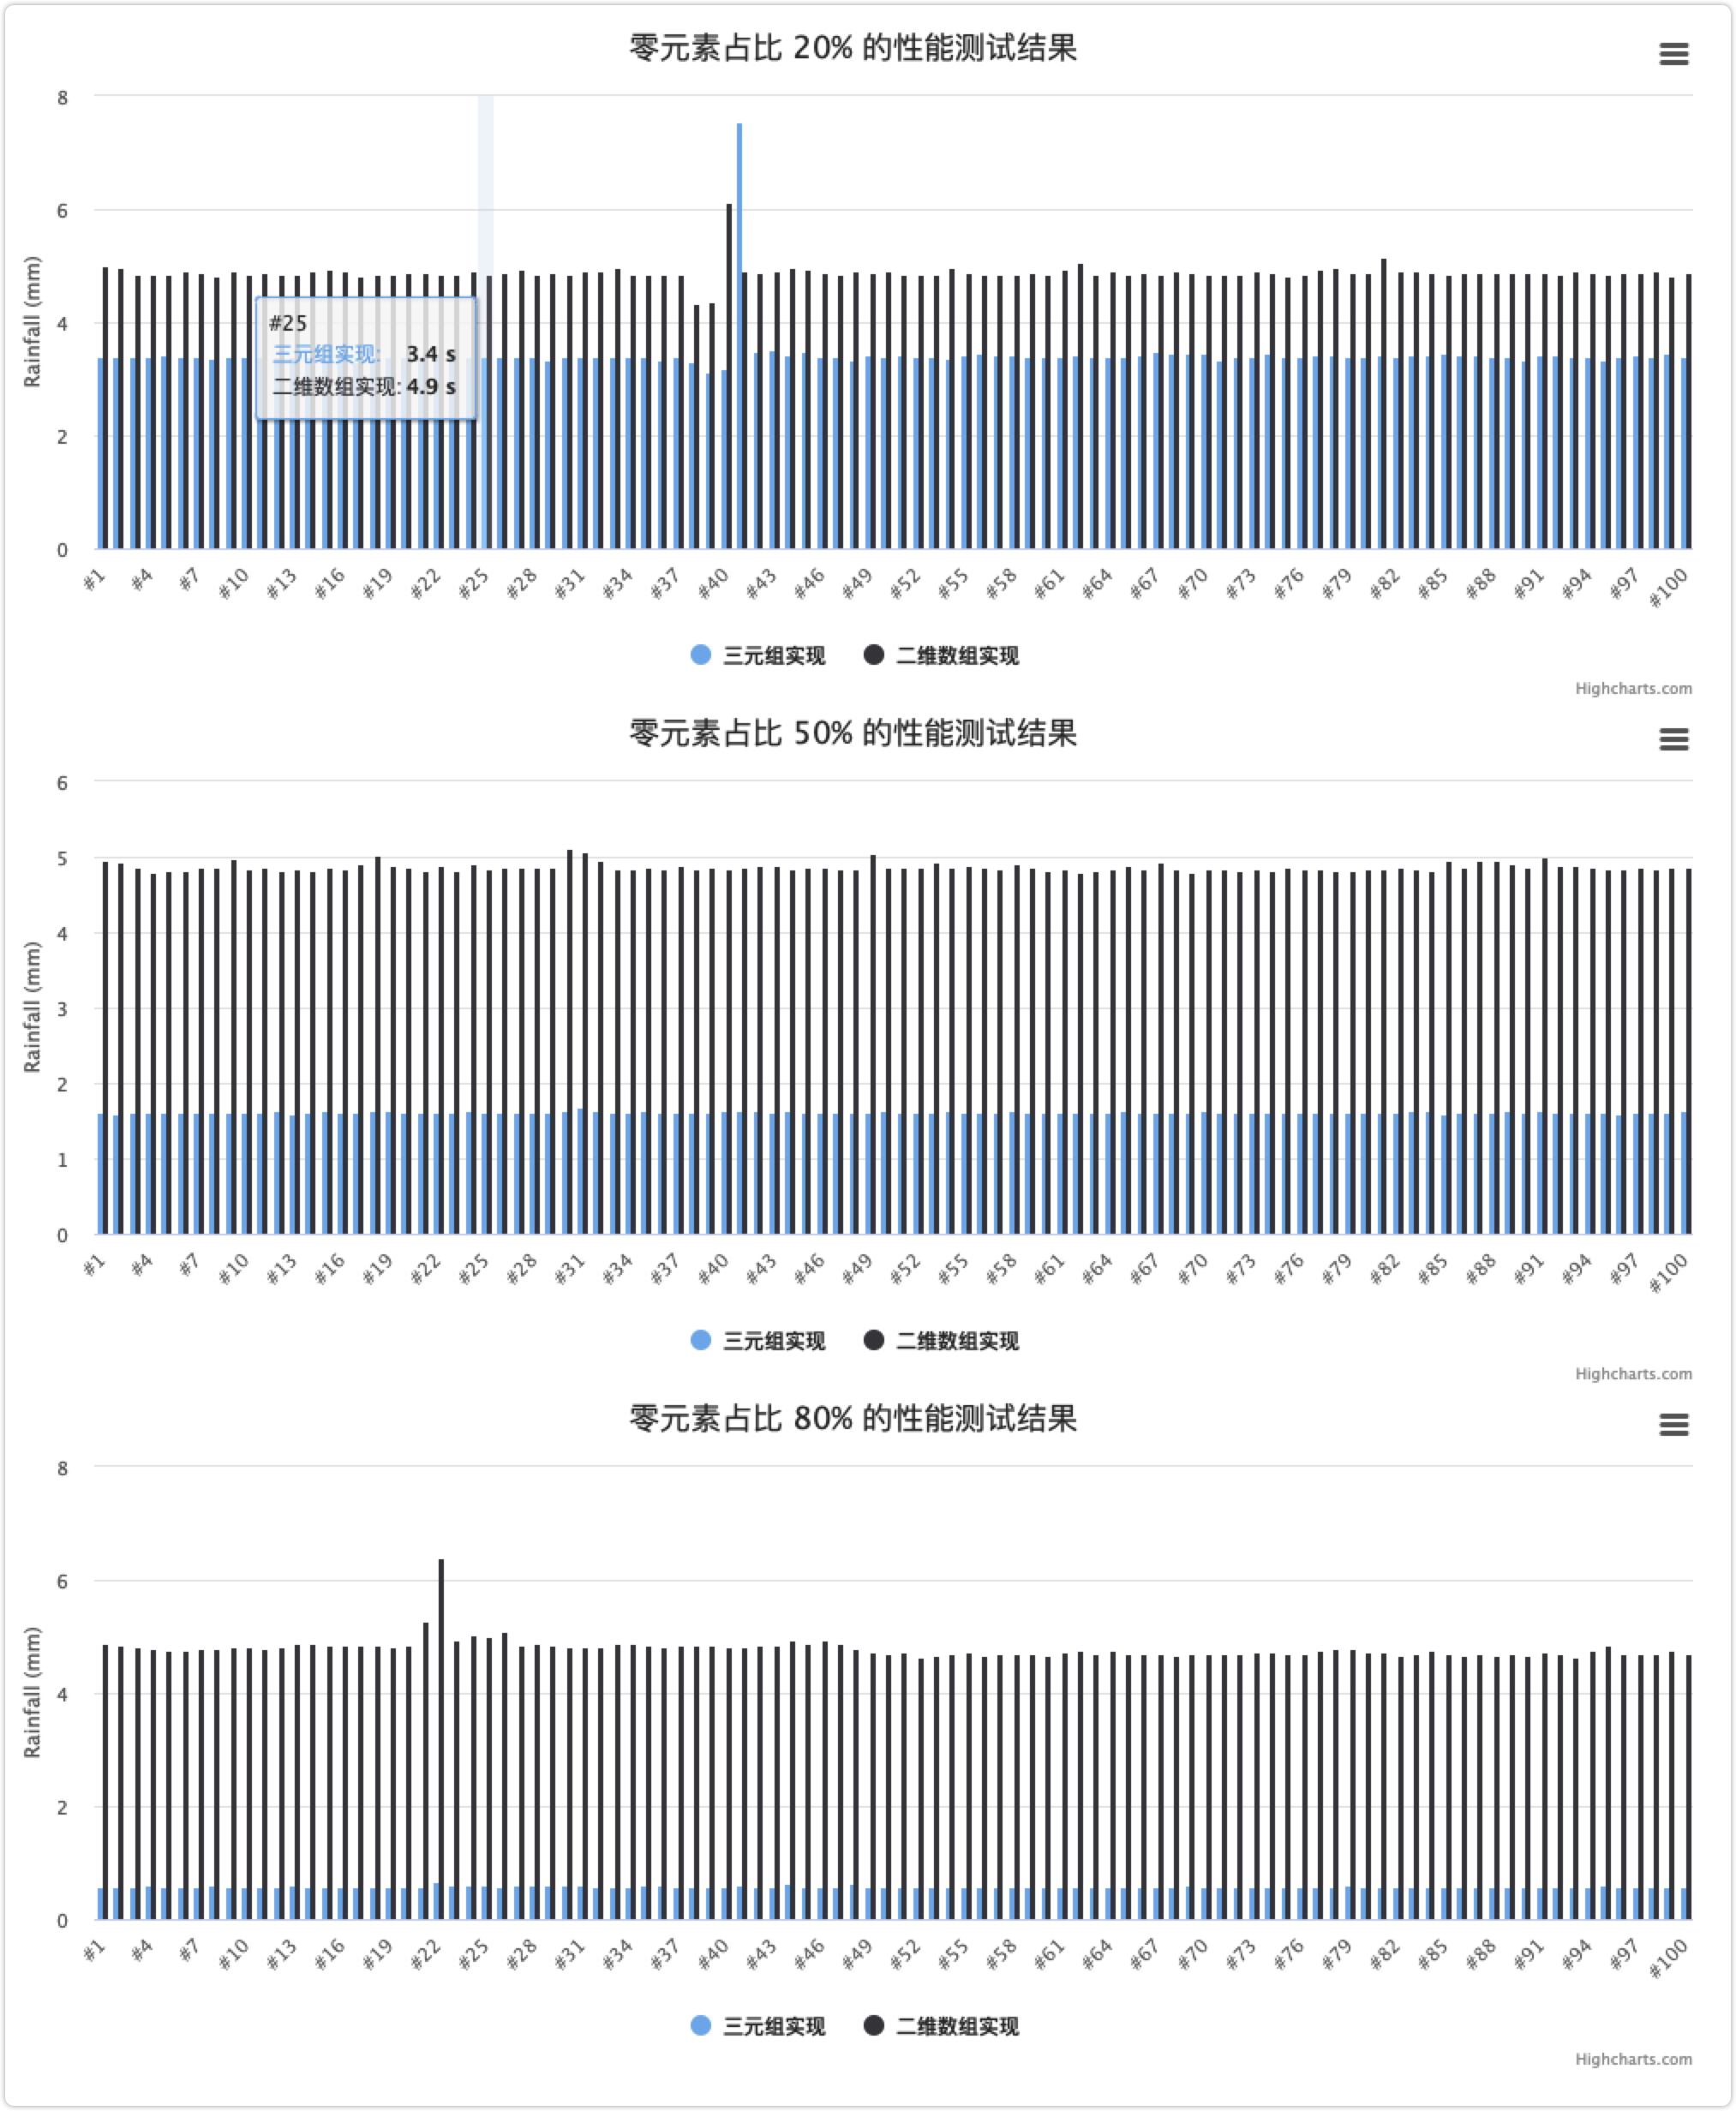
\includegraphics[width=0.9\textwidth]{./Images/pic3_3.png}
    
    \caption{可视化示例}
    
\end{figure}

\subsubsection{结论}

可以看出在规模较大的数据中,相比二维数组的实现,三元组表的实现在绝大多数情况下都有明显的性能优势,并且当矩阵越稀疏时性能优势越明显。

\end{document}
